% -*- root: ../main.tex -*-
% -*- dic: en_GB  -*-
\chapter{State of the art\label{sec:estado_del_arte}}

\paragraph{Abstract}

We cover here some of the basics needed to understand the real thesis of this \thisworkm. We will describe some fundamentals of the first order logic (\gls{FOL}), about his undeciability and, of course, how we can use the \gls{FOL} to prove properties of a program. Just two general properties will be covered, such as safety and liveness.

The thesis of this \thisworkm is the definition of a theory for linked list with which we can prove safety. Thus, we will define safety and some examples of how one can prove safety in simpler integer programs.

We include a brief logic of temporal logic needed for lifeness proving, but this topic is not very important in this \thisworkm.

Finally, we try to answer the question of parallelism. We will cover how can we prove safety for programs with multiple threads. We will describe some very important results used in this \thisworkm 
done by \citep{thesisAle}.

\section{First order logic}

\paragraph{Notation}
\label{def:notation}
We assume the usual way of representing and working with \gls{FOL}, this is
\begin{itemize}
	\item \textbf{Symbols:} $\{),(, \implies, \dimplies, \orcond , \andcond \}$
	\item \textbf{Quantifiers:} $\{\forall, \exists\}$
	\item \textbf{Constants:} $\{\true,\false\}$
	where we define $\true$ as \textit{true} and $\false$ as \textit{false}.
\end{itemize}

One could consider $\exists x(P(x))$  as an abbreviation of $\neg (\forall x(\neg P(x)))$, but for better understanding we would use both quantifiers when needed.
We could also use $(a \orcond b)$ instead of $(\neg a \implies b)$ but, again, for the better understanding those abbreviations will be used.
The same happens with $\true \equiv \neg \false$, but it is clearer when we use both symbols and not just one of them.


\paragraph{Definitions}

We are going to define some very basic concepts, needed and used during the whole \thisworkmp.

We say a formula $F$ is \concept{satisfiable} \gls{iff} there exists an interpretation $I$ such that $I \vDash F$. 
%
We say a formula $F$ is \concept{valid} \gls{iff} for all interpretations $I$, $I\vDash F$.
\label{def:validity}
This 2 concepts are very important and they are very related. $F$ is valid \gls{iff} $\neg F$ is unsatisfiable. 


A first-order \concept{theory} is defined by the following components: 
\begin{itemize}
	\item Its \textbf{signature} $\Sigma$ is a set of constant, function and predicate symbols.
	\item Its set of \textbf{axioms} $\axioms$ is a set of \gls{FOL} closed formula in which only elements from $\Sigma$ appear.
\end{itemize}



There are some important properties than a theory may have. 

A theory $\Sigma$ is \concept[Completeness]{complete} \gls{iff} for every closed $\Sigma-$formula $\sigma$ we have $(\Sigma\vDash \sigma) \orcond (\Sigma\neg\vDash \sigma) $

A theory $\Sigma$ is \concept[Consistency]{consistent} if there is at least one $\Sigma-$interpretation.	Equivalently, a theory $\Sigma$ is consistent if $\Sigma \not\vDash \false$

If our theory is not consistent, we can have a formal proof of anything we want to prove. 
%
We can prove contradictions. 
%
We could prove that some program is both correct and incorrect, which gives us no information. 
%
Thus consistency is a fundamental property for this \thisworkm.

In the other hand, completeness is very desirable, but may not be possible to achieve because of the incompleteness theorem of Gödel.


\begin{theorem}[Gödel's\IS incompleteness theorem]


For any formal effectively generated theory T including basic arithmetical truths and also certain truths about formal provability, if T includes a statement of its own consistency then T is inconsistent.


\textit{Obtained from \citeapos{Godel}}
\end{theorem}

% TODO: 
\todo{Conclusions}



It is not possible to have a complete and consistent theory while including basic arithmetical truths. 
%
One could expect that the theory needed to proof programs correctness wouldn't be complete. 
%
In that case, we will not be able to proof the incorrectness of a program.
%
Normally, consistency is basic while completeness is only desirable.

Another property of theories is the \textbf{decidability}. We say a theory $\Sigma$ is \concept{decidable} if $\Sigma \vDash F$ is decidable, for every $\Sigma-$formula 
and 
$F$ a $\Sigma-$formula is decidable if there is an \textbf{algorithm} that \textbf{always terminates} with ``yes'' if $F$ is valid in $\Sigma$ ($\Sigma$-valid) or ``no'' if $F$ is not $\Sigma-$valid.


Decidability is a stronger property of a theory than completeness. 
%
As completeness, decidability is a very desirable property but because \gls{FOL} (the theory with no axioms) is undecidable in general, we may not have decidability in the theory we are working on.



\begin{example}[\concept{Theory\IS of equality}]

\label{theory:equality}

We are going to define the theory of equality, because it is the simplest first-order theory.

The signature of the theory is:

\[\Sigma_e:\{=,a,b,c,...\}\]

and it's axioms are:

\begin{description}
	\item[Reflexivity:	] $\forall x, x=X$
	\item[Symmetry:	] $\forall x,y x=y \implies y=x$
	\item[Transitivity:	] $\forall x,y,z x=y \andcond y=z \implies x=z$
	\item[Function congruence:] For each function $f$
	\[\forall \gor{x},\gor{y} \left( \bigwedge_{i=1}^n x_i = y_i \right) \implies f(\gor{x}) = f(\gor{y})\]
	\item[Predicate congruence:]  For each predicate $P$
	\[\forall \gor{x},\gor{y} \left( \bigwedge_{i=1}^n x_i = y_i \right) \implies f(\gor{x}) \dimplies f(\gor{y})\]

	This 2 ``axioms'' are not axioms but an \concept[Axioms schema]{axiom schema}, because there is one axiom for each function $f$ or predicate $p$.
\end{description}

\gls{FOL} with equality is a decidable theory as Leopold Löwenheim proved in 1915 \cite{EqualityIsDecidable}. It is consistent and complete.
\end{example}


\subsection{Second-order logic (SOL)}

In \gls{SOL} the quantifiers can be used related to functions and/or predicates. This gives lot of possibilities to reason about the universe and problems but adds lot of complexity. 

In the theory of equality (\ref{theory:equality}) we could have defined axioms of congruence by:

\[\forall f \left( \forall \gor{x},\gor{y} \left( \bigwedge_{i=1}^n x_i = y_i \right) \implies f(\gor{x}) = f(\gor{y}) \right)\]
\[\forall P \left( \forall \gor{x},\gor{y} \left( \bigwedge_{i=1}^n x_i = y_i \right) \implies P(\gor{x}) \dimplies P(\gor{y}) \right)\]

This is a simpler way of writing but a more complex way of reasoning.

The \gls{SOL} is a very powerful tool in order to express formulaes. 
%
However, because it is not possible to reason automatically in theories of second order, we haven't used any second-order logic and we won't get deeper into it. 



\section{Program correctness}

We are finally ready to apply this concepts to a real word problem. In this \thisworkm we apply those concepts to prove some properties of programs.
%
The remaining task is to define the framework and the conventions we use to prove formally properties of programs.

There are two forms of proving properties. 
%
\concept{Partial\IS correctness} which assert that certain states can not occur during an execution (typically error states) or 
\concept{Total\IS correctness} which assert that some state is eventually reached during any execution. 
%
For total correctness we will have to introduce what \textbf{temporal logic} is and its quantifiers \textit{always} and \textit{eventually}. 
%
We will not go deep into temporal logic, because we will focus on partial correctness.




\label{def:SPL}
% -*- root: ../main.tex -*-
\subsection{Formal representation of a program}

This \gls{SPL} and its formal representation is the language chosen to write the programs to be formally verified.
%
It has been chosen by \citep{thesisAle} because its simplicity and \doubt{expressiveness} in order to write concurrent programs. 
%
Because its simplicity it is a great option to do formal verification with it.


\subsubsection{Preliminaries (Notation, definition)}

One can consider a program as a series of state changes. There are some variables, we execute one line of the program and some of those variables changes and some others don't. Thus, we can consider any program as a graph of states with some ways. For example, lets take a very simple program:
%
\[
	\begin{array}{l@{\hspace{0.3em}}c@{\hspace{1em}}l}
	\hline
		l_1 & : & \mathtt{x := -2} \\
		l_2 & : & \mathtt{\textbf{if } (x<0)} \\
		l_3 & : & \mathtt{\;\;x = 2x} \\
		l_4 & : & \mathtt{\textbf{...}}\\
	\hline
	\end{array}
\]
\label{simple:example}

This simple program doesn't do anything interesting, but it is useful to illustrate.
%
In figure \ref{ex:simpleExample} the directed graph of states is shown.

\begin{figure}[hbtp]
\label{ex:simpleExample}
\centering
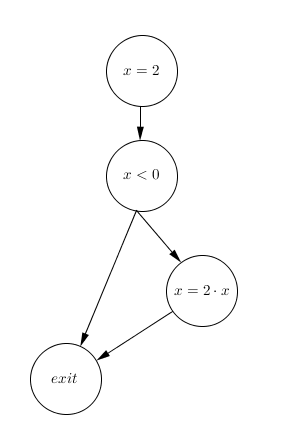
\includegraphics[scale=0.6]{graphics/simpleExample.png}
\caption{Directed graph of the program \ref{simple:example}}
\end{figure}


In the execution of this program, it is not possible to execute line 3 just after line 1 skipping line 2. We need to go line by line, respecting the execution flow. 
This is represented by the variable \pc (\concept{Program\IS counter}). This variable indicates the line to execute next.

So the state of the program at the beginning is 
%
\[ \pc = 1\]
%
This formula give all the information we have of the execution state. 
We know the \pc\; and the state and value of all variables (there are no more variables than \pc).

Now we need to define the step. 
%
How can we represent the execution of a line.
%
We need to use \concept{post-state} variables. 
%
We define the prime version of any variable to refer that same variable after the execution of the line (transition). 
%
Going back to the example, we have:
%
\[
\pc = 1 \andcond \pc'=2 \andcond x'=2 
\]

We have a post-state program counter ($\pc'=2$) and some post-state variables. 
%
As the execution of the assignment the variable $x$ takes a value (independently of the value in the pre-state), then $x'=2$ (regardless what value $x$ had). 

The next step could be
\[
\pc = 2 \andcond x'=x \andcond 	\pc'=?
\]

Where ? depends on the validity of the \textit{if} condition. 

This steps we have illustrated are called transition relations.

\begin{defn}[Transition relation]
A transition relation is the formula that define the step from one state of the program to another.  
\end{defn}

With this simple example, we have shown what a program counter and what a transition relation are. Now we can define the possible instructions a program may have.\footnote{We have just took the set of instructions the programs we are going to proof have.}

\subsubsection{Possible instructions}
As we are going to work with programs used by more than one thread, we need one program counter for each thread executing. 
%
We parametrize the program counter. 
%
This is, defining the \textbf{program counter} as a \textbf{function} that given a thread, returns its program counter. 
%
We could have define as one variable per thread, but it would be equivalent. 

For this definitions we use the letter $T$ to refer a particular thread.

\begin{description}
\item [Assignments:]
		The transition relation for a variable assignment consists of the 
		update of the program counter for the running thread and the 
		corresponding modification to the variable being assigned.
%
			\[
			\begin{array}[t]{p{8em}@{\hspace{6em}}p{\longtablesize}}
				\hline
				Statement & Transition relation \\ \hline\hline
				$\begin{array}[t]{l@{\hspace{0.3em}}c@{\hspace{1em}}l}
					l_1 & : & \mathtt{v := 2} \\
					l_2 & : & \mathtt{\cdots}
				\end{array}$
				&
				$\begin{array}[t]{ll}
					 \pc(T) = l_1 \andcond
					 \pc'(T) = l_2 \andcond
					 \mathtt{v}' = 2
				 \end{array}$ \\ 
				 \hline
			\end{array}
			\]
%
	\item [Pointer access:]
		Structure fields are accessible through the pointer operator \pointsto.
%
		There are two possible scenarios for the use of pointers, depending on 
		whether the statement accesses or modifies a structure field.
%
		We present now the semantics for both cases.
%
		The first case corresponds to the access of a structure field through an 
		address pointer.
%
\[
\begin{array}[t]{p{8em}@{\hspace{6em}}p{\longtablesize}}
	\hline
	Statement & Transition relation \\ \hline\hline
	$\begin{array}[t]{l@{\hspace{0.3em}}c@{\hspace{1em}}l}
		\ell_1 & : & \mathtt{v := a \pointsto field} \\ \\
		\ell_2 & : & \mathtt{\cdots}
	\end{array}$
	&
	$\begin{array}[t]{ll}
		 \pc(T) = \ell_1 \andcond
		 \pc'(T) = \ell_2 \andcond \\
		 \mathtt{v}' = \heap[\mathtt{a}].\mathtt{field}
	 \end{array}$ \\
	 \hline
\end{array}
\]
%
		The second case corresponds to the modification of a structure field using 
		an address pointer.
%
		Note how, in the second case, all structures (except the one pointed by 
		$\mathtt{b}$) remain unchanged.
%
		Also, all fields of the structure pointed by $\mathtt{b}$ remain unmodified 
		except for $\mathtt{field_n}$.
%
		\[
		\begin{array}[t]{p{8em}@{\hspace{6em}}p{\longtablesize}}
						\hline
						Statement & Transition relation \\ \hline\hline
						$\begin{array}[t]{l@{\hspace{0.3em}}c@{\hspace{1em}}l}
							\ell_1 & : & \mathtt{b \pointsto field_n := a} \\ \\ \\ \\
							\ell_2 & : & \mathtt{\cdots}
						\end{array}$
						&
						$\begin{array}[t]{ll}
							\pc(T) = \ell_1 \andcond \pc'(T) = \ell_2 & \andcond \\
							\heap' = \heap \{ \mathtt{b} \leftarrow c \} & \andcond \\
							c.\mathtt{field_n} = \mathtt{a} & \andcond \\
							\bigwedge\limits_{i \neq \mathtt{n}} c.\mathtt{field}_i = 
							\heap[\mathtt{b}].\mathtt{field}_i
						\end{array}$\\ \hline
			\end{array}
		\]

	\item [Conditionals:]
		We present now the two possible kinds of conditional statements in 
		SPL.
%
		In the first case, if condition $c$ does not hold, the execution 
		proceeds from the statement following the end of the conditional.
%
		\[
        \begin{array}[t]{p{8em}@{\hspace{6em}}p{\longtablesize}}
				\hline
				Statement & Transition relation \\ \hline\hline
				$\begin{array}[t]{l@{\hspace{0.3em}}c@{\hspace{1em}}l}
					\ell_1 & : & \mathtt{\textbf{if } c \textbf{ then }} \\ \\
					\ell_2 & : & \mathtt{\cdots} \\
						&& \mathtt{\vdots} \\
					\ell_n & : & \mathtt{\textbf{end if}} \\
					\ell_{n+1} & : & \mathtt{\cdots}
				\end{array}$
				&
				$\begin{array}[t]{ll}
					(\pc(T) = \ell_1 \andcond \;\;\mathtt{c} \andcond \pc'(T) = \ell_2) \; \Or \\
					(\pc(T) = \ell_1 \andcond \lnot \mathtt{c} \andcond \pc'(T) = \ell_{n+1})
				 \end{array}$ \\ \hline
			 \end{array}
		 \]
%
		In the second case, if condition $c$ does not hold, the execution 
		continues at the first statement in the \textbf{else} section of the 
		conditional statement.
%
		\[
				\begin{array}[t]{p{8em}@{\hspace{6em}}p{\longtablesize}}
				\hline
				Statement & Transition relation \\ \hline\hline
				$\begin{array}[t]{l@{\hspace{0.3em}}c@{\hspace{1em}}l}
					\ell_1 & : & \mathtt{\textbf{if } c \textbf{ then }} \\ \\
					\ell_2 & : & \mathtt{\cdots} \\
					\mathtt{\vdots} \\
					\ell_n & : & \mathtt{\textbf{else}} \\
					\ell_{n+1} & : & \mathtt{\cdots} \\
					\mathtt{\vdots} \\
					\ell_m & : & \mathtt{\textbf{end if}} \\
					\ell_{m+1} & : & \mathtt{\cdots}
				\end{array}$
				&
				$\begin{array}[t]{ll}
					(\pc(T) = \ell_1 \andcond \;\;\mathtt{c} \andcond \pc'(T) = \ell_2) \; \Or \\
					(\pc(T) = \ell_1 \andcond \lnot \mathtt{c} \andcond \pc'(T) = \ell_{n+1})
						& \text{for line } \ell_1 \\ \\ \phantom{\vdots} \\

						\pc(T) = \ell_n \andcond \pc'(T) = \ell_{m+1} & \text{for line } \ell_n
				 \end{array}$ \\ \hline
			\end{array}
		\]
%
	\item [Loops:]
		We consider the only loop statement available in SPL which executes 
	the statements in the body as long as the loop condition holds.
%
		\[
				\begin{array}[t]{p{8em}@{\hspace{6em}}p{\longtablesize}}
				\hline
				Statement & Transition relation \\ \hline\hline
				$\begin{array}[t]{l@{\hspace{0.3em}}c@{\hspace{1em}}l}
					\ell_1 & : & \mathtt{\textbf{while } c \textbf{ do }} \\
					\ell_2 & : & \mathtt{\cdots} \\
					\mathtt{\vdots} \\
					\ell_n & : & \mathtt{\textbf{end while}} \\
					\ell_{n+1} & : & \mathtt{\cdots}
				\end{array}$
				&
				$\begin{array}[t]{ll}
						(\pc(T) = \ell_1 \andcond \;\;\texttt{c} \andcond \pc'(T) = \ell_2) \; 
						\Or \\
						(\pc(T) = \ell_1 \andcond \lnot \texttt{c} \andcond \pc'(T) = 
					\ell_{n+1})
					& \text{for line $\ell_1$} \\ \\
					\pc(T) = \ell_n \andcond \pc'(T) = \ell_1 &
						\text{for line $\ell_n$}
				 \end{array}$ \\ \hline
			 \end{array}
		\]
%
			\item [Non deterministic choice:]
		The transition relation for the non-deterministic choice statement can 
		be expressed as follows:
%
		\[
			\begin{array}[t]{p{8em}@{\hspace{6em}}p{\longtablesize}}
				\hline
				Statement & Transition relation \\ \hline\hline
				$\begin{array}[t]{l@{\hspace{0.3em}}c@{\hspace{1em}}l}
					\ell_1 & : & \mathtt{\Nondet} \\
					\ell_2 & : & \mathtt{\;\;\;\;\;\; \cdots} \\
					\ell_3 & : & \mathtt{\textbf{or } \; \cdots} \\
					\mathtt{\vdots} \\
					\ell_n & : & \mathtt{\textbf{or } \; \cdots} \\
					\ell_{n+1} & : & \mathtt{\NondetEnd} \\
				\end{array}$
				&
				$\begin{array}[t]{ll}
					\pc(T) = \ell_1 \andcond
					\bigvee\limits_{i = 2..n} \pc'(T) = \ell_i
				 \end{array}$ \\ \hline
			 \end{array}
		\]
%
	\item [Lock and unlock:]
	Even though these are not SPL statements, as they will be widely used, it is necessary to define theirs transition relations.
%
		\[
			\begin{array}[t]{p{8em}@{\hspace{6em}}p{\longtablesize}}
				\hline
				Statement & Transition relation \\ \hline\hline
				$\begin{array}[t]{l@{\hspace{0.3em}}c@{\hspace{1em}}l}
					\ell_1 & : & \mathtt{\fLock(l)} \\
					\ell_2 & : & \mathtt{\cdots}
				\end{array}$
				&
				$\begin{array}[t]{ll}
					\pc(T) = \ell_1 \andcond
						\mathtt{l} = \oslash \andcond
						\mathtt{l}' = T \andcond \pc'(T) = \ell_2
				 \end{array}$ \\ \hline\hline
				$\begin{array}[t]{l@{\hspace{0.3em}}c@{\hspace{1em}}l}
					\ell_1 & : & \mathtt{\fUnlock(l)} \\
					\ell_2 & : & \mathtt{\cdots}
				\end{array}$
				&
				$\begin{array}[t]{ll}
					\pc(T) = \ell_1 \andcond
						\mathtt{l}' = \oslash \andcond \pc'(T) = \ell_2
				 \end{array}$ \\ \hline
			 \end{array}
		\]
%
\end{description}


% TODO: Mention the assume.
\subsection{Partial correctness (Safety)}

A function (or the whole program) is \textbf{partially correct} if when the function's precondition is satisfied on entry, its postcondition is satisfied when the function returns (if it ever does).
%
We present the \textbf{inductive assertion method} for proving partial correctness.


Let $\tau$ be the \gls{FOL} property to study. 
%
The procedure is the following:
%
First each function is reduced to a finite set of \gls{FOL} formulae called \concept[Verification condition]{\gls{VC}}.
%
\footnote{This reduction is done with the basic reducing cases we studied in \ref{def:SPL}.}
%
We achieve to prove that $\tau$ is valid in every state of the execution.
%
\textbf{Induction} is the methodology used.
%
First, we assert $\tau$ is valid before the program starts (induction base).
%
Then, we assume $\tau$ in the precondition and prove $\tau'$ valid.



Some examples are studied next to clarify the procedure.

\begin{example}
We study the loop version of the factorial function. We achieve to proof two formulae.

\[\tau_1 \equiv (l_5 \to \mathtt{x}\geq 1)\]

\[\tau_2 \equiv \mathtt{x} \geq 0\]


\caption{Loop version of the factorial function.}

\todo{Format}
\[
	\begin{array}{l@{\hspace{0.3em}}c@{\hspace{1em}}l}
	\hline
		l_1 & : & \mathtt{x := 10} \\
		l_2 & : & \mathtt{f := 1} \\
		l_3 & : & \mathtt{\textbf{while } (x\geq 1) \textbf{ do }} \\
		l_4 & : & \mathtt{	f = f*x} \\
		l_5 & : & \mathtt{	x=x-1} \\ 
		l_6 & : & \mathtt{\textbf{end while}}\\
		l_7 & : & \mathtt{\cdots}
	\end{array}
	\hline
\]
\label{simple:example}


First, we reduce the program to its \VC.


\[
	\begin{array}{l}
		 \psi_1 \equiv\pc(T) = l_1 \andcond \pc'(T) = l_2 \andcond \mathtt{f'=f} \andcond \mathtt{x}' = 10\\
		 \psi_2 \equiv\pc(T) = l_2 \andcond \pc'(T) = l_3 \andcond \mathtt{f}' = 1 \andcond x'=x\\
		 \psi_3 \equiv\pc(T) = l_3 \andcond \pc'(T) = l_4 \andcond \mathtt{f'=f} \andcond x'\geq 1\\
		 \psi_4 \equiv\pc(T) = l_4 \andcond \pc'(T) = l_5 \andcond \mathtt{f}' = \mathtt{f*x} \andcond \mathtt{x'=x}\\
		 \psi_5 \equiv\pc(T) = l_5 \andcond \pc'(T) = l_3 \andcond \mathtt{f'=f} \andcond \mathtt{x'=x-1}\\
		 \psi_6 \equiv\pc(T) = l_3 \andcond \pc'(T) = l_7 \andcond \mathtt{f'=f} \andcond \mathtt{x<1}
	\end{array}
\]

We need to prove, for $i=1,2$:

\[
	\left\{
		\begin{array}{l}
			\psi_1 \andcond \tau_i \to \tau_i'\\
			\psi_2 \andcond \tau_i \to \tau_i'\\
			\psi_3 \andcond \tau_i \to \tau_i'\\
			\psi_4 \andcond \tau_i \to \tau_i'\\
			\psi_5 \andcond \tau_i \to \tau_i'\\
			\psi_6 \andcond \tau_i \to \tau_i'\\
		\end{array}
	\right.
\]

\begin{center}\rule{4cm}{0.4pt}  $\tau_1$  \rule{4cm}{0.4pt}\end{center}
	
	\[
		\left(
			\underbrace{\pc(T) = l_1 \andcond \pc'(T) = l_2 \andcond \mathtt{f'=f} \andcond \mathtt{x}' = 10}_{\psi_1} \andcond \left(\underbrace{\pc(T) = l_5 \to \mathtt{x}\geq 1}_{\tau_1}\right)
		\right) 
				\to\left(\underbrace{\pc'(T) = l_5 \to \mathtt{x}' \geq 1}_{\tau_1'}\right)\\\\
	\]

	This formula is valid because $\pc(T) = l_2 \neq l_5$ thus the $\tau'_1$ is true.

	\[
		\left(
			\underbrace{\pc(T) = l_2 \andcond \pc'(T) = l_3 \andcond \mathtt{f}' = 1 \andcond x'=x}_{\psi_1} \andcond \left(\underbrace{\pc(T) = l_5 \to \mathtt{x}\geq 1}_{\tau_1}\right)
		\right) 
			\to\left(\underbrace{\pc'(T) = l_5 \to \mathtt{x}' \geq 1}_{\tau_1'}\right)\\\\
	\]

	This formula is valid because $\pc(T) = l_3 \neq l_5$ thus the $\tau'_1$ is true.

	\[
		\left(
			\underbrace{\pc(T) = l_3 \andcond \pc'(T) = l_4 \andcond \mathtt{f'=f} \andcond x'\geq 1}_{\psi_1} \andcond \left(\underbrace{\pc(T) = l_5 \to \mathtt{x}\geq 1}_{\tau_1}\right)
		\right) 
			\to\left(\underbrace{\pc'(T) = l_5 \to \mathtt{x}' \geq 1}_{\tau_1'}\right)\\\\
	\]
		This formula is valid because $\pc(T) = l_4 \neq l_5$ thus the $\tau'_1$ is true.

	\[
		\left(
			\underbrace{\pc(T) = l_4 \andcond \pc'(T) = l_5 \andcond \mathtt{f}' = \mathtt{f*x} \andcond \mathtt{x'=x}}_{\psi_1} \andcond \left(\underbrace{\pc(T) = l_5 \to \mathtt{x}\geq 1}_{\tau_1}\right)
		\right) 
			\to\left(\underbrace{\pc'(T) = l_5 \to \mathtt{x}' \geq 1}_{\tau_1'}\right)\\\\
	\]

	This formula is equivalent (applying resolution) to

	\[
		\left(
			\mathtt{x'=x} \andcond  \mathtt{x}\geq 1
		\right) 
		\to \left(\mathtt{x}'\geq 1)
	\]

	Which is valid because of equality congruence.

	\[
		\left(
			\underbrace{\pc(T) = l_5 \andcond \pc'(T) = l_3 \andcond \mathtt{f'=f} \andcond \mathtt{x'=x-1}}_{\psi_1} \andcond \left(\underbrace{\pc(T) = l_5 \to \mathtt{x}\geq 1}_{\tau_1}\right)
		\right) 
			\to\left(\underbrace{\pc'(T) = l_5 \to \mathtt{x}' \geq 1}_{\tau_1'}\right)\\\\
	\]

	This formula is valid because $\pc(T) = l_3 \neq l_5$ thus the $\tau'_1$ is true.

	\[
		\left(
			\underbrace{\pc(T) = l_3 \andcond \pc'(T) = l_7 \andcond \mathtt{f'=f} \andcond \mathtt{x<1}}_{\psi_1} \andcond \underbrace{\pc(T) = l_5 \to \mathtt{x} \geq 1}_{\tau_1}
		\right) 
			\to \left(\underbrace{\pc'(T) = l_5 \to \mathtt{x}' \geq 1}_{\tau_1'}\right)\\\\
	\]

	This formula is valid because $\pc(T) = l_7 \neq l_5$ thus the $\tau'_1$ is true.


\paragraph{Conclusion:} we have proven that $\pc(T) = l_5 \to x \geq 1$. 
%
This is called an \concept[Invariant]{invariant} because it is true during all the execution. 
%
This transition has been chosen specially because it is needed in the proof of $\tau_2$.

\begin{center}\rule{4cm}{0.4pt}  $\tau_2$  \rule{4cm}{0.4pt}\end{center}

	\[
		\left(
			\underbrace{\pc(T) = l_1 \andcond \pc'(T) = l_2 \andcond \mathtt{f'=f} \andcond \mathtt{x}' = 10}_{\psi_1} \andcond \underbrace{\mathtt{x} \geq 0}_{\tau_2}
		\right) 
				\to  \underbrace{\mathtt{x}' \geq 0}_{\tau_2'}\\\\
	\]

	This formula is valid because $x'=10 \to x'\geq 0$.

	\[
		\left(
			\underbrace{\pc(T) = l_2 \andcond \pc'(T) = l_3 \andcond \mathtt{f}' = 1 \andcond x'=x}_{\psi_1} \andcond \underbrace{\mathtt{x} \geq 0}_{\tau_2}
		\right) 
			\to \underbrace{\mathtt{x}' \geq 0}_{\tau_2'}\\\\
	\]


	This formula is valid because of the congruence of equality used in  $x'=x \andcond x\geq 0 \to x'\geq 0$ 

	\[
		\left(
			\underbrace{\pc(T) = l_3 \andcond \pc'(T) = l_4 \andcond \mathtt{f'=f} \andcond x'\geq 1}_{\psi_1} \andcond \underbrace{\mathtt{x} \geq 0}_{\tau_2}
		\right) 
			\to \underbrace{\mathtt{x}' \geq 0}_{\tau_2'}\\\\
	\]

	This formula is valid because $x'\geq 1 \to x'\geq 0$.

	\[
		\left(
			\underbrace{\pc(T) = l_4 \andcond \pc'(T) = l_5 \andcond \mathtt{f}' = \mathtt{f*x} \andcond \mathtt{x'=x}}_{\psi_1} \andcond \underbrace{\mathtt{x} \geq 0}_{\tau_2}
		\right) 
			\to \underbrace{\mathtt{x}' \geq 0}_{\tau_2'}\\\\
	\]

	This formula is valid because of the congruence of equality used in  $x'=x \andcond x\geq 0 \to x'\geq 0$ 

	\[
		\left(
			\underbrace{\pc(T) = l_5 \andcond \pc'(T) = l_3 \andcond \mathtt{f'=f} \andcond \mathtt{x'=x-1}}_{\psi_1} \andcond \underbrace{\mathtt{x} \geq 0}_{\tau_2}
		\right) 
			\to \underbrace{\mathtt{x}' \geq 0}_{\tau_2'}\\\\
	\]

	This formula has some more difficulty. 
	%
	Because we are inside the loop $x$ should be greater than 1.
	%
	However, we don't have that information in the formula.
	
	The solution is use some \concept{support}.
	%
	A support formula is a formula added to the precedent of an implication to give more information. 
	%
	This addition does not change the validity of the formula.
	%
	We could equivalently prove

	\[
		\psi_i \andcond \tau_1 \andcond \tau_2 \to \tau_2' \leftrightarrow \psi_i\andcond \tau_2\to\tau_2'
	\]

	And this is exactly the solution to proof this \gls{VC}

	\[
		\left(
			\underbrace{\pc(T) = l_5 \andcond \pc'(T) = l_3 \andcond \mathtt{f'=f} \andcond \mathtt{x'=x-1}}_{\psi_1} \andcond \underbrace{\mathtt{x} \geq 0}_{\tau_2} \andcond \underbrace{\pc(T) = l_5 \to \mathtt{x} \geq 1}_{\tau_1}
		\right) 
			\to \underbrace{\mathtt{x}' \geq 0}_{\tau_2'}\\\\
	\]

	And this formula is valid. Applying resolution we get an equivalent valid formula:

	\[
		\left( \mathtt{x'=x-1} \andcond \mathtt{x'}\geq 1\right) \to \mathtt{x} \geq 0
	\]



	\[
		\left(
			\underbrace{\pc(T) = l_3 \andcond \pc'(T) = l_7 \andcond \mathtt{f'=f} \andcond \mathtt{x<1} \andcond \mathtt{x'=x} }_{\psi_1} \andcond \underbrace{\mathtt{x} \geq 0}_{\tau_2}
		\right) 
			\to \underbrace{\mathtt{x}' \geq 0}_{\tau_2'}\\\\
	\]

	This formula has some more difficulty too.
	%
	One can think that the unique possible value of $x$ should be $0$ because of the content of the loop.
	%
	However, that information is not within the formula.
	%
	As we did before, some support is needed to prove this formula.
	%
	The support needed is $\tau_3 \equiv \pc(T) = l_3 \to \mathtt{x} \geq 0$.
	%
	The proof of this invariant is not included because it does not give new relevant information. 
	%
	Using this invariant, we have:

	\[

		\left(
			\underbrace{\pc(T) = l_3 \andcond \pc'(T) = l_7 \andcond \mathtt{f'=f} \andcond \mathtt{x<1} \andcond \mathtt{x'=x}}_{\psi_1} \andcond \underbrace{\mathtt{x} \geq 0}_{\tau_2} \andcond \underbrace{\pc(T) = l_3 \to \mathtt{x}\geq 0 }_{\tau_3}
		\right) 
			\to \underbrace{\mathtt{x}' \geq 0}_{\tau_2'}\\\\
	\]
	
	And this formula is valid. Applying resolution we get an equivalent valid formula:

	\[
		\left(
			\mathtt{x'=x}  \andcond \mathtt{x}\geq 0 \to \mathtt{x'}\geq 0
		\right)
	\]


\end{example}

\begin{example}
\todo{Multiple thread partial correctness example}
\end{example}




\subsection{Total correctness (Lifeness)}

\todo{Complete with Césars Book}
What is proving lifeness, for what we need temporal logic.

\subsubsection{Temporal logic}

Basics on temporal logics

Temporal logic studies problems like the one exposed below.

\begin{example}
\label{Collatz:conjecture}

Let $f$ be the following function.

\[
f(n) = \left\{
	\begin{array}{cc}
		\rfrac{n}{2} & \text{ if } (n\text{ mod } 2) \equiv 0\\
		3n+1 & \text{ if } (n\text{ mod } 2) \equiv 1
	\end{array}
\right.
\]

We can form a sequence applying repeatedly $f$. If we take the sequence starting in $n=13$ we get:

\[ 
	13 \overset{\displaystyle\;\; 3n+1\;\;}{\longrightarrow}
	40 \overset{\displaystyle\;\;\rfrac{n}{2}\;\;}{\longrightarrow}
	20 \overset{\displaystyle\;\;\rfrac{n}{2}\;\;}{\longrightarrow}
	10 \overset{\displaystyle\;\;\rfrac{n}{2}\;\;}{\longrightarrow}
	5 \overset{\displaystyle\;\; 3n+1\;\;}{\longrightarrow}
	16 \overset{\displaystyle\;\;\rfrac{n}{2}\;\;}{\longrightarrow}
	8 \overset{\displaystyle\;\;\rfrac{n}{2}\;\;}{\longrightarrow}
	4 \overset{\displaystyle\;\;\rfrac{n}{2}\;\;}{\longrightarrow}
	2 \overset{\displaystyle\;\;\rfrac{n}{2}\;\;}{\longrightarrow}
	1
\]

One could ask if this sequence eventually stops regardless the integer chosen to begin. This question is called \concept{Collatz conjecture} and has not been solved yet. 
For the moment, an infinite sequence has not been found, but the temporal logic problem has not been proven either.

The temporal formula for this problem is:

\todo{Formula of conjecture}
\[

\]


\end{example}


\subsection{Parametrized systems}

The correctness of just one thread executing a program is easy because it runs sequentiality.
%
Multiple threads executing the same program is a different and more difficult problem to solve.
%
If the number of threads executing is not bounded is another important and difficult step.
%
If the number of threads is bound, one could unroll the formula for all the threads in the problem and try to prove it. 
%
This is why we focus the unbounded case, which is the usual scenario.
\todo{Examples?}


We are going to study those cases. 
%
To do so, we need to parametrize the program executed by multiple threads. Typically the threads would be $i$,$j$,$k_0$,$k_1$,... 



\subsubsection{Arbitrary number of threads}

\todo{Reread paper of parametrized systems and rewrite}

For example, the web servers may not have a bound of the number of clients they can accept.
%
Can we prove correctness when an unbounded number of processes are using the same shared variable?

A recent research \citeapos{paperParametrizedInvariants} has proven a very important result. 
%
We will enunciate it and discuss it because it is fundamental for this work.


\begin{theorem}[Bound an arbitrary number of threads]
We just need to prove 3 things. Initiation, self consecution and others consecution.
\todo{Real enunciate}
\end{theorem}
\label{thm:biggest}

Using this powerful result, we have reduced an arbitrary number of processes sharing the same variable to a finite number of threads sharing the variable. 
%
This is a very powerful result and we will come to it later on, when we talk about the proofs we have done. 

We illustrate the power of this theorem with the next example:

\begin{example}
\todo{Example. From the paper?}
\end{example}

